\chapter{State of the Art of Tools for Autonomous Vehicles} \label{sec:related-work}

\section{Dataset}

The progress of autonomous driving has been driven by the availability of large-scale datasets that capture the complexity and variability of real-world environments. These datasets have evolved from early perception-focused collections to multimodal, interactive, and reasoning-centered benchmarks. This section reviews the main real-world datasets outlining their contributions, scope, and how they progressively address the challenges of perception, interaction, planning, and reasoning in autonomous driving.

Early efforts like the KITTI dataset \cite{geiger2013} laid the foundation for ADV perception research by providing multimodal sensor data, including stereo cameras, LiDAR, and high-precision GPS/IMU. KITTI captured over 6 hours of diverse driving scenarios, covering urban, rural, and highway environments, and introduced benchmarks for stereo vision, optical flow, 3D object detection, SLAM, and visual odometry\cite{geiger2012,geiger2013} but has the drawback of being limited to one city only.

KITTI was the most complete dataset at that time \cite{kang2019}, laying the foundation for many others to come. An extensive number of other open datasets in the real world before 2019 can be found in the survey by \cite{kang2019} and a more up-to-date review of available datasets can be found in \cite{liu2021} and \cite{liu2024}. Up to 2019 there were no major changes in public available datasets until Waymo published the data collected by their ADV prototype. However, a few intermediate datasets introduced significant improvements in scope and data richness compared to KITTI.

The ApolloScape dataset, developed by Apollo Auto, an open source autonomous driving division from the Chinese giant Baidu, expanded beyond KITTI by combining high-resolution RGB videos, dense 3D point clouds, and centimeter-level localization with fine-grained semantic and instance annotations \cite{Huang_2018_CVPR_Workshops}. Provided pixel-accurate labels for more than 28 classes, including vehicles, lane markings, and traffic signs, in varied lighting and weather conditions. This broader diversity and label density addressed KITTI’s limited scale and single-city coverage.

The Berkeley DeepDrive Video (BDDV) dataset \cite{Xu_2017_CVPR}, created by the University of California, Berkeley, introduced a large-scale video collection with GPS/IMU data and driver action signals. Unlike KITTI’s frame-based setup, BDDV offered continuous driving sequences supporting temporal modeling and end-to-end learning for behavior prediction. 

Based on the BDDV dataset, BDD100K \cite{Yu_2020_CVPR} significantly expanded the scale and diversity of Berkeley’s driving data, introducing 100K video clips with comprehensive annotations for ten heterogeneous tasks, including object detection, segmentation, lane detection, tracking, and imitation learning. BDD100K emphasized multitask learning in visual and temporal domains.

The nuScenes dataset \cite{Caesar_2020_CVPR} was one of the first large-scale multimodal benchmarks that combined LiDAR, radar, cameras, and HD maps for urban perception tasks. It enabled 3D detection, tracking, and sensor fusion research in diverse traffic conditions in Boston and Singapore. The Waymo Open Dataset (WOD) \cite{sun2020} extended this concept, offering significantly greater scale, geographic diversity, and annotation density. WOD integrates data from full-scale autonomous prototypes with high-precision localization and large-scale LiDAR coverage. 

%The first contribution from Waymo was the perception dataset mentioned above, but one year after its release they also made available a motion dataset \cite{waymo_open_dataset} that included more than 100,000 segment of map data. In 2025 the end-to-end driving dataset with more than 2,000 runs was released \cite{waymo_open_dataset} showing a new trend to apply this strategy in recent ADV prototypes.

In the next year Waymo made available its waymo open motion dataset (WOMD) \cite{ettinger2021} later upgraded with LiDAR data \cite{chen2024} , extending its previous release to motion forecasting. This dataset focuses on predicting the future trajectories of multiple interacting agents such as vehicles, pedestrians, and cyclists. %It contains more than 100,000 scenes, each 20 seconds long at 10 Hz, collected across six US cities, totaling more than 570 hours of driving data.
Unlike earlier datasets, it explicitly labels interactive scenarios and supports joint prediction tasks, enabling the development of models for multi-agent motion forecasting.

Demonstrating the wide adoption of WOD, community-driven research has produced several augmented datasets based on WOD and WOMD to address specialized perception and reasoning challenges. At the geometric and motion level, the Scene Flow dataset \cite{jund2021scalable} and OmniNOCS \cite{10.1007/978-3-031-73226-3_8} expand perception capabilities beyond object detection. Scene flow augments WOD v1.2 with dense 3D motion vectors per point, enabling large-scale supervised scene flow estimation. OmniNOCS introduces a unified 3D Normalized Object Coordinate Space across over 90 object classes, including Waymo data, providing instance masks and 3D bounding boxes for geometry-aware monocular perception.

At the behavioral and interaction level, the CausalAgents benchmark \cite{sun2024causalagents} and the ROAD-Waymo dataset \cite{khan2024road} enhance understanding of agent dynamics and context. CausalAgents adds human-verified causal labels identifying influential agents and perturbed validation splits for robustness studies. ROAD-Waymo extends WOD with dense action, agent type, and location annotations for large-scale event detection and situational awareness tasks.

As research moved beyond isolated perception, the focus shifted toward cooperative and communication-based datasets. Earlier real-world cooperative perception datasets such as V2V4Real \cite{Xu_2023_CVPR} and V2X-Real \cite{10.1007/978-3-031-72943-0_26} provided synchronized LiDAR and camera data for studying multi-agent perception across connected vehicles. The DeepSense-V2V dataset \cite{11029591} introduces a comprehensive real-world benchmark centered on vehicle-to-vehicle communication and cooperative perception. Unlike traditional single-vehicle datasets, it integrates synchronized mmWave communication data with multimodal sensing—including LiDAR, radar, 360-degree cameras, and GPS—captured in realistic driving scenarios. This combination enables exploration of sensing-assisted communication tasks such as beam alignment, blockage prediction, and cooperative localization. DeepSense-V2V tries to bring together autonomous perception and next-generation communication systems, trying to provide the bases for developing 6G-enabled cooperative driving intelligence.

Although most large-scale real-world datasets focus on common driving conditions, the Corner Case Dataset \cite{smartcities8040129} targets rare, safety-critical situations that are underrepresented in existing benchmarks. Constructed from multisource naturalistic driving data, including vehicle mounted sensors, drone recordings, and tachograph accident videos, it introduces a quantitative framework for identifying low-probability, high-risk events. Each scenario is standardized using the OpenSCENARIO format, facilitating simulation-based testing and benchmarking of the robustness of autonomous vehicles. 

Building on these advances in perception and cooperation, the nuPlan dataset \cite{10610077} extends the nuScenes framework and introduces the first large-scale benchmark for learning-based planning. 
NuPlan provides a full stack environment for testing planning algorithms under realistic interactions. It enables the assessment of both open-loop and closed-loop performance, bridging the gap between data-driven motion forecasting and decision making for autonomous driving.


Taking advantage of the latest advances in large language models (LLMs), the WOMD Reasoning dataset \cite{li2024womd} adds natural language annotations to WOMD, with nearly three million question–answer pairs describing maps, trajectories, and interactions. This connects perception and motion prediction with language-based reasoning, forming the largest open corpus for multimodal understanding in autonomous driving.

Extending LLM-based reasoning beyond single-vehicle understanding, the V2V-LLM dataset \cite{chiu2025v2vllmvehicletovehiclecooperativeautonomous} explores cooperative driving scenarios through multimodal language reasoning. Built on real V2V perception datasets such as V2V4Real and V2X-Real, it enables question–answering tasks across connected autonomous vehicles, encompassing object identification, cooperative planning, and occlusion reasoning. By integrating natural language with shared sensory data, V2V-LLM demonstrates how LLMs can coordinate multiple agents and infer intent between vehicles, expanding the scope of multimodal reasoning to collaborative driving.

The latest Waymo release was its end-to-end driving dataset \cite{hwang2025emma}, which also integrates LLM into the autonomous driving pipeline. EMMA unifies perception, prediction, and planning within a single multimodal framework by mapping raw sensor and textual inputs into structured driving outputs. Built on WOD and WOMD, it uses LLM reasoning to generate interpretable driving decisions and achieve state-of-the-art results on nuScenes and competitive performance on Waymo benchmarks.

This last approach revives interest in end-to-end driving, since NVIDIA’s pioneering DAVE-2 system \cite{bojarski2016endendlearningselfdriving}, now reimagined through the reasoning and scalability capabilities of modern multimodal LLMs.

\subsection{Synthetic Datasets}

Real-world data collection can be expensive, time-consuming and challenging to scale \cite{feng2020}. Furthermore, real-world datasets often suffer from a long-tail distribution of scenarios, where rare but critical events such as accidents and unusual weather conditions are rarely presented \cite{song2024}. Gathering more data and corner cases is becoming more critical than inventing new deep neural network architectures. Collecting such data in the real world can be dangerous or infeasible. 

Therefore, synthetic datasets offer a cost-effective and scalable alternative, allowing researchers to create customized scenarios and accelerate their research results. However, this introduces a new set of challenges: ensuring that synthetic data accurately reflect the complexities of the real world, including sensor noise, object textures, and physical dynamics. The evolution of synthetic datasets for ADV is well surveyed by \cite{song2024}. We will explore the most relevant synthetic datasets revealed by the cited survey and other relevant datasets found in academic databases.

Before modern simulators, early synthetic datasets such as Virtual KITTI \cite{Virtual_kitti} and SYNTHIA \cite{Ros_2016_CVPR} supported only image-based perception tasks such as segmentation and depth estimation. Although useful for pretraining and domain adaptation, their lack of multimodal sensing and realistic agent interaction limited their applicability to full autonomous driving systems.

The introduction of modern 3D engines such as Unity \cite{unity_engine} and Unreal Engine \cite{unreal_engine} transformed synthetic data generation by enabling photorealistic rendering, dynamic lighting, and physically accurate scene composition. Building on these advances, the introduction of the Carla simulator \cite{Dosovitskiy2017} in 2018 utilized Unreal Engine to offer a new systematic approach to performance testing and dataset creation in autonomous driving contexts. It was developed partially by the same authors of the Synthia Dataset release one year earlier. 

Since its debut, the Carla simulation platform, along with its comprehensive sensor suites, has enabled the easy synthesis of additional datasets, thanks to its realistic, adaptable, and open-source design. Furthermore, it allowed the easy creation of virtual ADV prototypes as close to the real ones as possible. The majority of the  multimodal synthetic ADV datasets found in the literature applies the Carla as a generation tool.

The IDDA, SHIFT, and EMS3D-KITTI datasets take advantage of Carla to create a multimodal perception system. IDDA \cite{Alberti2020Idda:Driving} introduced synchronized RGB and depth data with semantic and instance labels, while SHIFT \cite{Sun2022SHIFT:Adaptation} extended this concept to multi-sensor setups including LiDAR, depth, and multi-camera imagery. More recently, EMS3D-KITTI \cite{Jaiswal2025EMS3D-KITTI:Training} further enhanced the classical KITTI framework by synthesizing dense 3D point clouds and RGB cameras within a CARLA environment, supporting cross-domain training for detection and depth estimation. The last one focuses on emergency vehicle detection such as ambulance and police vehicles trying to bridge the gap on rare objects detection.

%ParisCARLA-3D \cite{deschaud2021} uses the same LiDAR camera mapping setup in real Paris streets and inside CARLA, creating paired synthetic and real point clouds with shared semantic and instance labels. It supports three core 3D tasks—semantic segmentation, instance segmentation, and scene completion—and is designed to evaluate how well models transfer from synthetic to real outdoor environments.

%Moreover, Carla-Gear \cite{Nesti2024CARLA-GeAR:Models} focuses on robustness. It generates driving data for segmentation, monocular depth, and 2D/3D detection, but incorporates physical adversarial patches placed on billboards or trucks. These patches are produced through white-box optimization and embedded directly into the rendered scenes, creating controlled test sets for benchmarking adversarial vulnerability in autonomous-driving perception.

Robustness and domain-transfer datasets include Paris-CARLA-3D \cite{deschaud2021} and Carla-GeAR \cite{Nesti2024CARLA-GeAR:Models}. Paris-CARLA-3D pairs synthetic and real LiDAR–camera captures using identical sensor layouts to study transferability and cross-domain consistency in 3D segmentation and scene completion. Carla-GeAR focuses on robustness testing by embedding physically inspired adversarial perturbations directly into Carla-rendered scenes to evaluate model vulnerability under controlled attacks.

%Using the Carla simulator for a different approach, SKoPe3D \cite{Pahadia2023SKoPe3D:Cameras} focuses on infrastructure-based perception and provides synthetic roadside camera data for vehicle keypoint estimation. It extends the simulator with a procedural keypoint-generation pipeline that assigns consistent 3D semantic keypoints to vehicles in diverse layouts, lighting, and weather. It targets structural cues instead of bounding boxes or masks.

SKoPe3D \cite{Pahadia2023SKoPe3D:Cameras} provides a synthetic dataset specifically for vehicle keypoint perception from roadside cameras, addressing limitations in existing traffic monitoring benchmarks that focus on ego-vehicle views. It is generated using the CARLA simulator with a roadside perspective and includes per-vehicle annotations such as bounding boxes, tracking IDs, and 33 semantic keypoints per instance. It was designed to support 3D keypoint and pose estimation.


Using the Carla environment, OPV2V  and V2X-Sim  explored synthetic cooperative perception in the context of integrating vehicle-to-vehicle (V2V) and vehicle-to-infrastructure (V2I). OPV2V \cite{xu2022opv2vopenbenchmarkdataset} focuses on V2V perception, capturing more than 70 realistic traffic scenarios under varying occlusion and communication delay conditions and in the evaluation of cooperative fusion strategies. V2X-Sim \cite{Li2022V2X-Sim:Driving} couples CARLA with SUMO \cite{behrisch2011sumo} to record synchronized data from multiple vehicles and roadside units, offering multimodal streams from RGB cameras, LiDAR, GPS and IMU, with ground truths for collaborative detection, tracking, and segmentation. 

Being the only synthetic cooperative dataset to not use Carla as its data source as exposed in its paper, LSTV-V2V \cite{Suo2024LSTV-V2V:Perception} instead uses Prescan \cite{prescan2025} and CityEngine \cite{cityengine2025}. It constructs large-scale traffic scenes derived from real urban maps via OpenStreetMap, combining camera and LiDAR data across various types of road and weather conditions. LSTV-V2V focuses on large-scale, customizable Vehicle-to-Vehicle cooperation scenarios that support dynamic scene synthesis with realistic environmental diversity.

In an effort to tackle critical long tail challenging scenarios, NVIDIA released along with its generation tool the Cosmos-Drive-Dreams dataset \cite{Ren2025Cosmos-Drive-Dreams:Models}. Instead of Carla, it used Nvidia Cosmos \cite{nvidia_cosmos} to generate driving scenarios from real world recordings for the dataset. It has HDMap information, LiDAR point clouds, and calibrated camera views. It derives synthetic clips from real data labels, allowing diverse weather and illumination variations that are difficult to capture at scale in the real world, expanding long-tail coverage of existing real-world datasets.



\section{Workload Characterization}

Workload characterization is the process of empirically measuring, analyzing, and modeling inputs processed by a computing system to understand their properties, dynamics, and impact on system performance \cite{Calzarossa2016WorkloadRevisited}. In the context of autonomous vehicles, workload characterization is particularly challenging due to the complexity of the software stack, tight real-time constraints, and the strong dependence of computation on environmental conditions and sensor input.

The initial work by \citeonline{Liu2017} characterized the ADV computation to motivate heterogeneous designs, describing the general architecture of autonomous vehicles and matching each type of workload to specific processing units. %\citeonline{Lin2018} extend this line by analyzing bottlenecks in a real-time autonomous-driving system and comparing acceleration options. This work established tail latency as a critical metric for autonomous driving workloads and demonstrated the need to analyze full pipelines rather than isolated components.
\citeonline{Lin2018} extend this line by implementing an end-to-end autonomous driving system and characterized its workload by instrumenting perception, localization, planning, and control components to measure execution time and latency while processing realistic sensor data.

Benchmark suites often include empirical measurement of autonomous driving workloads through predefined execution pipelines and systematic performance evaluation. CAVBench \cite{wang2018} define a benchmark suite for ADV computing and report both application-facing results, reflecting the performance of autonomous driving pipelines, and system-facing outcomes, capturing the behavior of the underlying computing platform. Chauffeur \cite{Maity2021Chauffeur:Systems} includes an initial characterization of end-to-end pipeline response times on embedded platforms by measuring end-to-end execution latency, illustrating how workload composition affects latency. ADBench \cite{Tabani2022ADBench:Systems} follows a comparable approach by defining benchmark pipelines for autonomous driving systems and reporting execution-time and performance metrics obtained through controlled benchmark execution.

In industry, ADASMark \cite{EEMBC2019ADASMark} provides a standardized ADAS-oriented vision-centric pipeline benchmark, focusing on end-to-end performance behavior for comparative evaluation across platforms.  Edge AIBench \cite{Hao2022EdgeSystems} adopts a scenario-driven benchmarking methodology that includes autonomous driving workloads as part of a broader IoT–Edge–Cloud evaluation, reporting end-to-end latency and resource utilization through the execution of predefined pipelines. These efforts characterize workloads through the execution and measurement of benchmark-defined pipelines, capturing computational behavior at the pipeline and system levels without performing explicit analysis of workload variability.

Subsequent studies focused on detailed end-to-end characterization of open-source autonomous driving frameworks. \citeonline{Becker2020DemystifyingSystems} presented a comprehensive workload characterization of Autoware, measuring per-module latency, end-to-end latency, and power consumption under realistic sensor inputs. %Their analysis showed that contention between concurrently executing modules and LiDAR-intensive components significantly impacts latency and predictability, and that profiling modules in isolation substantially underestimates real execution times. 
Similarly, \citeonline{Alcon2020TimingSolutions} characterized the timing behavior of the Apollo autonomous driving stack by collecting execution-time traces for individual components over extended executions, allowing statistical analysis of execution-time distributions and variability. %statistically characterized the variability in the execution time of the Apollo autonomous driving stack, showing that execution times exhibit wide distributions and strong jitter between modules.
\citeonline{Alcon2023MainThem} later investigated the underlying sources of such variability and non-determinism by including the software structure examination, proposing a taxonomy that distinguishes algorithmic, architectural, and platform-level factors influencing execution-time behavior. %Their analysis showed how data-dependent behavior, internal randomization, and data-flow dependencies can amplify variability across the pipeline.


Some studies have concentrated on characterizing perception workloads, which are widely recognized as the dominant contributors to autonomous driving computation. \citeonline{Tang2022CharacterizationEdge} analyzed real-time object detection workloads on vehicular edge platforms, measuring CPU and GPU utilization, inference latency, and scalability across different deep learning models and frameworks. %Their results showed large differences in resource utilization and that only a subset of models meets real-time constraints, highlighting the importance of model-specific workload characterization. 
\citeonline{Tang2023PerceptionVehicles} and \citeonline{Feng2025CharacterizingComputing} characterized perception workloads in memory-constrained edge environments by measuring inference latency, execution-time distributions, and memory usage in different object detection models and deep learning architectures.

%Workload characterization has also been extended to capture dynamic and tail behavior under varying driving conditions. \citeonline{Liu2023COLA:Systems} conducted a systematic study of tail latency in Level-4 autonomous driving systems, showing that latency distributions are strongly influenced by traffic density and environmental complexity \cite{liu2023cola}. Their characterization revealed bursty computation patterns and mismatches between static pipeline configurations and dynamic latency requirements. Similarly, Liu et al. investigated inference-time variability in perception pipelines and identified the structure of deep neural networks and multi-tenant resource contention as primary causes of execution-time variation \cite{liu2022prophet}. These works reinforce the importance of characterizing distributions and tail behavior rather than relying on mean latency.

Workload characterization has also been extended to capture dynamic and tail behavior under varying driving conditions.  \citeonline{Liu2023COLA:Systems} characterized the Level-4 autonomous driving workloads by instrumenting a complete autonomous driving pipeline and collecting timestamped traces across consecutive frames while executing the system under controlled driving scenarios with varying traffic density and scene complexity. Their methodology records end-to-end execution latency from sensor input to control output, enabling the construction of latency distributions and the analysis of temporal workload dynamics. \citeonline{Liu2022Prophet:Vehicles} instrumented perception pipelines to characterize workload behavior by repeatedly measuring per-frame inference latency under different input conditions and execution environments. %Their methodology relies on detailed tracing of perception execution, including single-tenant and multi-tenant deployments, to capture execution-time variability and interference effects. Together, these works exemplify workload characterization approaches based on systematic tracing and repeated execution of autonomous driving software under controlled yet representative operating conditions.

More recently \citeonline{Pham2025ADPerf:Systems} characterized the performance of obstacle detection modules in Apollo and Autoware by measuring execution latency and service rates during pipeline execution, allowing analysis of how workload behavior propagates across dependent components. Their methodology emphasizes empirical measurement of execution behavior within realistic autonomous driving software stacks.

\section {Task Scheduling}
Task scheduling in autonomous driving systems concerns the allocation and ordering of computation across sensing, perception, planning, and control components under strict real-time constraints. Recent work therefore moves beyond isolated per-task timing constraints and instead treats scheduling as an integrated control problem over pipelines, data dependencies, and platform-level resource contention, with explicit attention to timing assurance, data timeliness, and safe degradation under overload.

As autonomous driving pipelines exhibit significant execution-time variability due to environmental conditions and input complexity, some authors explored runtime and middleware-level scheduling mechanisms. \citeonline{Bai2020} proposes AutoE2E, an adaptive real-time middleware for autonomous driving control that aims at meeting the requirements of the end-to-end deadline despite variations in execution-time, using coordinated mechanisms that adjust the execution behavior of the application online. AutoRS \cite{Ma2023} further incorporated environment-dependent scheduling by adjusting task rates and priorities based on driving context, using nested control loops to balance deadline satisfaction and resource utilization.

Complementarily, \citeonline{Gog2022} proposed a dynamic deadline-driven execution model in which deadlines are treated as first-class runtime entities that can change over time and trigger corrective actions when violated. The system enforces deadlines between fine-grained execution events and centralizes deadline management across pipeline stages. Along the same line, \citeonline{Ma2023HCPerf:Vehicles} proposed HCPerf, a performance-directed hierarchical coordination framework that schedules autonomous driving tasks based on runtime driving performance metrics, coordinating task execution rates and priorities to jointly improve end-to-end deadline satisfaction, control responsiveness, and throughput under execution-time variability.

Some studies represent autonomous driving software as task graphs in order to analyze its schedulability and overall end-to-end timing behavior. \citeonline{Sun2023} proposed a scheduling framework that models an autonomous driving system as a directed acyclic multi-rate graph, enabling joint analysis of task schedulability and end-to-end latency across sensing-to-actuation chains. Similarly, \citeonline{Yano2024} introduced a multi-deadline DAG scheduling model tailored to systems based on Autoware, decomposing end-to-end constraints into local relative deadlines for subgraphs and extending Global Earliest Deadline First algorithm to handle multiple deadlines within a single execution graph.

Beyond schedulability analysis, studies refine graph-based scheduling models to better reflect semantics specific to autonomous driving workloads. \citeonline{Xu2022} proposed an AoI-centric scheduling framework for autonomous driving systems, modeling sensing and processing tasks as a DAG and formulating scheduling decisions to minimize Age of Information at critical control points. \citeonline{Sobhani2025} addressed limitations of conventional DAG models by explicitly modeling different sensor fusion triggering patterns, including timer-driven, wait-for-all, and immediate fusion. Their formulation represents fusion behavior as scheduling constraints and generates deterministic schedules that optimize reaction time, time disparity, and freshness-related metrics.

The scheduling challenges in autonomous driving systems also arise from integration with automotive platforms and real-time software. \citeonline{Askaripoor2021} proposed a flexible scheduling architecture for autonomous driving platforms that separates planning and distribution functions, enabling adaptive resource allocation and reduced message drops under varying computational load. Similarly \citeonline{Yang2023} developed a parallel pruning approach to accelerate task scheduling in AUTOSAR-based systems, reducing the complexity of exploring feasible scheduling configurations under real-time constraints.

Other studies focus on the impact of heterogeneous computing platforms on task scheduling decisions. \citeonline{amarnath2021} proposed HetSched, a heterogeneity-aware scheduler for autonomous vehicles that dynamically prioritizes tasks across heterogeneous processing elements while preserving safety-critical timing constraints. Their approach explicitly considers execution-time differences between processing units and integrates task criticality into scheduling decisions. Extending this perspective, \citeonline{Han2025} proposed a fine-grained multi-XPU abstraction called XAUTO that decomposes autonomous applications into schedulable units and dynamically assigns them to heterogeneous devices based on performance and energy models, demonstrating improvements in end-to-end execution efficiency on heterogeneous platforms.

\citeonline{kairos} introduced Data-flow Availability as a mechanism to express and monitor timing requirements on data dependencies rather than on individual tasks. Their system detects violations of availability constraints at runtime and coordinates mitigation actions across scheduling layers, addressing timing errors that arise from buffering, asynchronous execution, and data propagation effects that are common in autonomous driving pipelines.

More recently, learning-based scheduling has also been explored at the operating system and task-management levels. \citeonline{Sethuraman2023AnSVM} proposed an intelligent task management system using adaptive support vector machine and heuristic optimization to assign autonomous driving tasks to heterogeneous processors based on CPU utilization and task urgency. Moreover, \citeonline{Seo2025SCHED:Vehicles} introduced SCHED, a safe CPU scheduling framework that makes use of reinforcement learning trained in an offline setting and translated into decision trees suitable for deployment at the operating-system level, targeting reductions in tail latency for mixed-criticality autonomous driving workloads.

In a related direction, \citeonline{Youssef2025TRATSS:Vehicles} proposed TRATSS, a transformer-based task scheduling system that models task dependencies using self-attention mechanisms to generate scheduling decisions for graph-based autonomous vehicle tasks, demonstrating the feasibility of deep learning for complex scheduling problems.

\section {Related Work}
Research tools for autonomous driving often focus on one part of the experimental loop: generating data and scenarios in simulation, characterizing system performance and bottlenecks, or enforcing timing constraints through scheduling and timing assurance. Several were listed in the previous section. However, in practice, these dimensions interact. The scenario configuration changes sensor streams and algorithm behavior, which changes compute demand and timing, which then affects whether deadlines can be met. 

Because Cart-OnePiece targets an integrated workflow (scenario configuration → dataset generation → workload characterization → scheduling-policy evaluation), the most relevant prior work is framework-level tooling that supports at least one, and preferably two or more, of these aspects in a reusable way. The following works that will be discussed next are listed in table \ref{tab:rw_aspects} and deal strongly with one aspect and at least partially with the other aspects of the ADV simulation.

%\paragraph{Summary of aspect coverage.}
%Table~\ref{tab:rw_aspects} summarizes the closest frameworks/tools found in the selected literature. We use ``Yes'' only when the paper explicitly claims that capability; otherwise, we mark it as ``Partial/Unclear''.

\begin{table}[t]
\centering
\footnotesize
\setlength{\tabcolsep}{3pt}
\renewcommand{\arraystretch}{1.15}
\caption{Related tools/frameworks vs. thesis aspects. ``Partial'' indicates the paper suggests the capability indirectly (e.g., simulator integration or timing models) but does not present it as a supported feature.}
\label{tab:rw_aspects}
\begin{tabularx}{\linewidth}{@{}>{\raggedright\arraybackslash}Xccc@{}}
\hline
\textbf{Tool / Framework} & \shortstack[c]{\textbf{Dataset}\\\textbf{Generation}} & \shortstack[c]{\textbf{Workload}\\\textbf{Characterization}} & \textbf{Scheduling} \\
\hline
Chauffeur~\cite{Maity2021Chauffeur:Systems} & No & Yes & Partial \\
Pylot~\cite{Gog2021Pylot:Vehicles} & Partial & Yes & Partial \\
D3 / ERDOS~\cite{Gog2022} & No & Partial & Yes \\
RT-MOT~\cite{Kang2022RTMOT:RTSS} & No & Yes & Yes \\
RTAS DAG ~\cite{Sun2023} & No & Partial & Yes \\
Kairos~\cite{kairos} & No & Partial & Yes \\
AD-TTS~\cite{Li2025ADTTS} & Yes & Partial & Partial \\
Cart-OnePiece (this work) & Yes & Yes & Yes \\
\hline
\end{tabularx}
\end{table}

Chauffeur \cite{Maity2021Chauffeur:Systems} is positioned as a benchmark suite for embedded systems researchers and designers who need to profile and characterize configurable end-to-end self-driving pipelines. A key contribution is that Chauffeur explicitly targets platform-aware analysis on embedded NVIDIA systems and provides code and profiling scripts to reproduce characterization. It also demonstrates how designers can evaluate timing behavior under shared resources and explore approaches like parallel execution to reduce end-to-end delay, and it discusses evaluating schedulability of representative self-driving workloads. 

However, Chauffeur is first and foremost a benchmark and characterization suite. Although it uses schedulability evaluation and delay-reduction as motivating demonstrations, it is not presented as a unified environment where users can systematically plug in and compare multiple scheduling policies across many simulated driving scenarios while simultaneously collecting dataset artifacts and resource traces.

Pylot \cite{Gog2021Pylot:Vehicles} presents a modular ADV platform built around a high-performance data flow representation, where the pipeline components are operators communicating with timestamped messages. The stated goal is to study latency–accuracy effects and how they influence end-to-end driving behavior, and Pylot provides reference implementations of common pipeline components and can connect to simulators such as CARLA, as well as real vehicles with minimal changes. 

Pylot partially addresses dataset generation because it can be configured to log sensor streams and internal-module outputs, and it includes perfect modules that obtain ground truth from CARLA and can generate new training data sets. It also partially addresses scheduling by offering a deterministic execution structure and timing-control mechanisms, but it does not position itself as a framework for systematically swapping and evaluating multiple scheduling policies.

\citeonline{Gog2022} propose D3 (Dynamic Deadline-Driven) as an execution model for autonomous vehicle pipelines where deadlines and runtime–accuracy tradeoffs vary with the driving context. The work centralizes deadline management and allows applications to react to missed deadlines modeled as exceptions, then describes ERDOS as an open-source framework that reveals detailed execution events and enables speculative execution, while still enforcing deadlines between any chosen events. The work also emphasizes the need for realistic ADV benchmarking and evaluates the approach by driving an ADV pipeline through challenging simulated scenarios.

RT-MOT \cite{Kang2022RTMOT:RTSS} introduces a real-time scheduling framework that incorporates confidence awareness for multiple multi-object tracking tasks under limited compute. It combines offline timing guaranties based on fixed-priority, non-preemptive baseline with the smallest workload configuration with runtime feasibility checks that enable taking on heavier workloads when there is available capacity. The paper is explicit about measurement as it uses an execution-time profiling approach and discusses GPU/CPU division of work.

RT-MOT is relevant as a concrete example of workload-adaptive scheduling in an autonomy-relevant perception component. Nevertheless, it is focused on multiple object tracking, not an end-to-end autonomous driving pipeline.

\citeonline{Sun2023} formulates an autonomous driving system as a multi-rate DAG and proposes an integrated framework to co-analyze schedulability and end-to-end latency constraints across task chains. In addition, it introduces integer linear programming techniques to guide the elimination of redundant workload to increase the likelihood of meeting the timing requirements. It partially characterizes the workload by measuring the computation time and the success ratio of its applied scheduling results.

\citeonline{kairos} targets autonomous cyber-physical systems (CPS) where timing violations cause safety risks. The paper proposes representing key temporal expectations such as freshness, consistency, and stability as timing constraints on data flows, then introduces Kairos to detect timing constraint violations at runtime via instrumentation and mitigate them through a cross-layer scheduling infrastructure. It is evaluated on multiple platforms including Autoware. it combines deep systems analysis and profiling (workload/timing bottlenecks) with runtime assurance mechanisms.

AD-TTS \cite{Li2025ADTTS} is explicitly positioned as both a simulation framework and a dataset for event prediction in time-triggered autonomous driving. The authors extend an autonomous driving simulation based on CARLA and ROS into a multi-task, time-triggered system and log events at each scheduling cycle together with metadata including timestamps, CPU utilization, and memory usage.

However, AD-TTS is not presented as a platform for comparing different runtime scheduling policies. Its schedule is produced offline and is kept fixed during runtime, meaning the framework is mainly a dataset and trace-generation platform intended to support research on prediction and later adaptation, rather than a scheduling experimentation environment.

Table~\ref{tab:rw_overview_tools_objectives} compares related works that propose tools and frameworks to evaluate key aspects of an ADV computing system (dataset generation, workload characterization, and task scheduling) and contrasts them with Cart-OnePiece. The table summarizes, for each work, the tool/technique adopted and its main objective.

\begin{table}[t]
\centering
\small
\setlength{\tabcolsep}{6pt}
\renewcommand{\arraystretch}{1.15}
\caption{Overview of related work, the tool/technique used, and the objective of each work.}
\label{tab:rw_overview_tools_objectives}
\begin{tabular}{p{0.22\linewidth} p{0.28\linewidth} p{0.45\linewidth}}
\hline
\textbf{Works} & \textbf{Tool} & \textbf{Objective} \\
\hline
(Maity et al., 2021) & \textit{Chauffeur} (benchmark suite) &
Enable end-to-end benchmarking and performance analysis of autonomous-driving (ADV) workloads on embedded systems. \\
\hline
(Gog et al., 2021) & \textit{Pylot} (modular ADV platform) &
Support experimentation on latency--accuracy tradeoffs by composing/swapping ADV pipeline components (often in simulation). \\
\hline
(Gog et al., 2022) & \textit{D3 / ERDOS} (deadline-driven runtime framework) &
Improve ADV pipeline behavior using dynamic deadlines and runtime support to meet timing goals under changing conditions. \\
\hline
(Kang et al., 2022) & \textit{RT-MOT} (real-time scheduling framework) &
Provide confidence-aware real-time scheduling for multi-object tracking to balance tracking quality and timing constraints. \\
\hline
(Sun et al., 2023) & \textit{RTAS multi-rate DAG framework} (timing-correctness framework) &
Guarantee timing correctness for ADV pipelines modeled as multi-rate DAGs (schedulability + end-to-end constraints). \\
\hline
(Li et al., 2024) & \textit{Kairos} (timing assurance system) &
Achieve timing assurance in autonomous/CPS dataflow pipelines via availability-aware runtime/system mechanisms. \\
\hline
(Li et al., 2025) & \textit{AD-TTS} (simulation framework + dataset) &
Provide a multi-task simulation framework and dataset for studying time-triggered/event-driven behavior in ADV workloads. \\
\hline
\textbf{Our work} & \textbf{Cart-OnePiece} (own tool/framework) &
Integrate simulation with a task-based heterogeneous runtime to unify dataset generation, workload characterization, and scheduling strategy evaluation for on-board ADV computation. \\
\hline
\end{tabular}
\end{table}

Based on the analysis of the related work and the key pillars introduced in the Background and State of the Art sections, it is possible to observe that none of the surveyed solutions offers a single integrated environment that simultaneously supports end-to-end experimentation on dataset generation, workload characterization, and scheduling strategy evaluation for onboard ADV computation. Instead, existing works typically emphasize one main capability and only partially address the others. Therefore, Cart-OnePiece stands out as a unique contribution by unifying these capabilities in one workflow, enabling reproducible ADV experiments and consistent comparisons under controlled simulated scenarios.

\begin{comment}
\subsection{Related Work}
\label{subsec:related_work}





\subsubsection{Simulation-based platforms that expose system-level behavior}
A first cluster of related work focuses on running full or partial AD pipelines in a modular form so that end-to-end behavior can be studied under different models, rates, and runtime conditions.

\paragraph{Pylot.}
Pylot (Gog et al., ICRA 2021) presents a modular ADV platform built around a high-performance dataflow representation, where pipeline components are operators communicating with timestamped messages. The stated goal is to study latency–accuracy effects and how they influence end-to-end driving behavior, and Pylot provides reference implementations of common pipeline components and can connect to simulators such as CARLA as well as real vehicles with minimal changes. This makes Pylot a strong reference for workload characterization focused on latency/accuracy tradeoffs at the pipeline level. However, Pylot is not presented as a dataset generation tool, and the paper does not position Pylot as a framework for designing and comparing scheduling policies (even if time budgeting is discussed as a need).

\paragraph{D3 and ERDOS.}
D3 (Gog et al., EuroSys 2022) targets the execution problem that arises when deadlines and runtime–accuracy tradeoffs vary with the environment. The paper proposes a deadline-driven execution model (D3) and implements ERDOS as an open-source realization for AD pipelines, explicitly emphasizing deadline specification/enforcement and mechanisms such as reacting to missed deadlines and exposing fine-grained execution events. In contrast to platforms that only evaluate static pipelines, D3/ERDOS is directly concerned with scheduling under dynamic deadlines and how the pipeline adapts its computation. Its evaluation uses an AV pipeline (including Pylot-based components) to study deadline allocation policies and the effects of static versus dynamic deadlines on system behavior. This work is therefore close to the thesis in terms of system-level scheduling and timing behavior, but it does not aim to integrate dataset generation (as an explicit capability) with scheduling experiments, nor does it present a user-facing environment for scenario-configurable dataset extraction linked to compute metrics.

\subsubsection{Benchmarking and workload characterization on embedded platforms}
A second cluster emphasizes benchmarking suites and instrumentation to characterize AD workloads, often motivated by embedded constraints.

\paragraph{Chauffeur benchmark suite.}
Chauffeur (Maity et al., ACM TECS 2021, presented at CODES+ISSS 2021) is a benchmark suite intended for embedded systems design and end-to-end analysis of self-driving workloads. The paper explicitly frames Chauffeur as enabling profiling and characterization of configurable end-to-end pipelines, and it includes characterization on representative embedded platforms and a use case showing how designers can reduce end-to-end delay via parallel execution. As such, Chauffeur is directly relevant to workload characterization and experimental evaluation on target-like hardware. Still, Chauffeur is primarily a benchmark suite and analysis vehicle; it is not described as a dataset generation framework, and while it discusses schedulability and end-to-end timing, it is not positioned as a general framework for implementing and comparing alternative scheduling strategies across scenarios in the way targeted by this thesis.

\paragraph{AD-TTS dataset and simulation framework.}
AD-TTS (Li, Onwuchekwa, Obermaisser; PDF metadata indicates 2025) is explicitly positioned as both a simulation framework and a dataset for event prediction in time-triggered autonomous driving. The authors extend an autonomous driving simulation based on CARLA and ROS into a multi-task, time-triggered system and log events at each scheduling cycle together with metadata including timestamps, CPU utilization, and memory usage. This makes AD-TTS one of the few works in the selection that clearly supports two of the thesis aspects at once: scenario-driven simulation that produces a dataset, and workload characterization signals tied to execution. The scheduling angle is present because the motivation is adaptive time-triggered systems and proactive/speculative scheduling driven by event prediction, but the paper’s primary contribution is the dataset/framework rather than an environment for systematically swapping and evaluating multiple on-board scheduling policies.

\subsubsection{On-board scheduling and timing assurance for autonomous workloads}
A third cluster focuses on scheduling methods and timing assurance, generally assuming the AD pipeline exists and asking how to guarantee (or improve) temporal correctness under constraints.

\paragraph{Kairos and data-flow availability.}
Kairos (Li \& Zhang, OSDI 2024) introduces Data-flow Availability (DFA) to express temporal properties such as freshness/consistency/stability as timing constraints on data flows, and proposes a programming model plus mechanisms to detect and mitigate timing-constraint violations. The paper explicitly includes cross-layer scheduling for mitigation and a profiler/annotation workflow to specify expected temporal properties. This is close to the thesis goal in the sense that it treats timing assurance as a system problem that spans software layers, but it does not address dataset generation and does not primarily target workload characterization as a reusable experimental workflow (beyond what is needed for detecting timing violations).

\paragraph{Multi-rate DAG scheduling for AD systems.}
Sun et al. (RTAS 2023) formulate an AD system as a multi-rate DAG and propose an integrated analysis framework to co-analyze task schedulability and end-to-end latency, including an ILP-based method that guides dropping redundant workload to increase the chance of meeting timing requirements. This work is highly relevant to system-level scheduling strategies for on-board pipelines, especially where tasks have different rates and complex dependencies. However, the contribution is an analysis-and-refinement framework rather than a simulation-based environment; it does not provide dataset generation or empirical workload characterization instrumentation as a central feature.

\paragraph{RT-MOT for perception workloads.}
RT-MOT (Kang et al.; PDF metadata indicates 2022) proposes a confidence-aware real-time scheduling design for multiple multi-object tracking tasks, motivated by the dual requirement of timely execution and high tracking accuracy under limited resources. Compared to pipeline-wide scheduling frameworks, RT-MOT is narrower in scope (tracking), but it is directly relevant as an example of scheduling that explicitly trades workload/quality against timing constraints in an autonomy-relevant perception component. Because it is component-focused, it does not cover dataset generation and does not present workload characterization as a general pipeline feature, but it provides a concrete scheduling pattern that a broader experimental framework can incorporate and evaluate.

\subsubsection{Positioning and gap relative to this thesis}
Across these works, two patterns emerge. First, platforms and benchmarks that facilitate measurement (e.g., Chauffeur, Pylot) typically stop short of offering scheduling as a configurable experimental dimension across many scenarios, and they rarely connect dataset extraction to the measured compute metrics in a reusable way. Second, scheduling and timing-assurance frameworks (e.g., D3/ERDOS, Kairos, Sun et al., RT-MOT) address temporal correctness and adaptation, but they commonly assume that inputs and datasets are external artifacts and do not provide an integrated workflow for scenario-configurable dataset generation coupled with workload characterization.

The tool developed in this thesis (CArt-OnePiece) is designed to close this gap by integrating (i) configurable simulation-driven dataset generation, (ii) empirical workload characterization (execution time, latency, and resource usage), and (iii) scheduling policy design and evaluation within a single reusable environment. In this sense, the closest prior art covers important subsets of the intended workflow, but none of the selected tools is presented as a unified experimental framework that simultaneously supports scenario-driven dataset extraction and systematic scheduling experimentation while producing directly comparable characterization measurements.

\begin{comment}

\subsection{AUTOSAR}

The Automotive Open System Architecture (AUTOSAR) is a association of companies from the automotive and software industry that aims to create a standardized automotive architecture and framework for the development of automotive software systems. That group was formed due to the increase of in system vehicle complexity leading to the necessity to create development standards to avoid the deadlocks caused by proprietary individual solutions. The AUTOSAR main objectives were the integration of functional modules from different suppliers, software scalability, network transfer of system functions, maintainability and software updates and upgrades through the product life time \cite{Furst2016}.

The AUTOSAR standards development started back in 2003 and in 2007 it was first released and applied in vehicle mass production. It moved from a Electronic Control Unit (ECU) based system to a function based system design. Nowadays, it is divided in classic and adaptive platforms. The classic platform was the standard for traditional vehicle functionalities. That was the first set of standards created to standardize the software used in the ECUs. With it was possible to promote decoupling of hardware and software for reuse, flexibility and scalability purposes. \cite{Langheim2014}. The abstraction layer was the main concept to promote the decoupling from the applications designed by programmers and the specific Original Equipment Manufactures (OEM) hardware. 

The ADV development pushed the hardware and software requirements one step further. So the AUTOSAR needed to evolve to follow this new reality. The adaptive platform was created to address the high computing power necessary to run the ADV complex AI algorithms keeping the automotive specific requirements already implemented in the classic platform \cite{AUTOSAR}. The main advances were the implementation of an operational system and a communication middleware allowing data exchange with in vehicle and external hardware. In addition, it has the support to integrate existing vehicle architectures that communicates using Ethernet. In the functional point of view the applications on the adaptive platform were free to create and kill tasks and to allocate memory with well defined boundaries different from the very rigid and fixed scheduling and memory management from the classic platform.

The set of rules described in the AUTOSAR standards allow to develop reliable car products that follows the description on it. All the development details are recorded in a description file especially the distributed system configuration. That configuration would include information such as software and system description and ECU configuration. That description file is valid for big car parts manufacturers but is a big overhead in the ADV research field \cite{Jo2014}. Furthermore, new studies in the ADV software architecture could lead to changes in the way that the description file information is recorded. Another drawback is the high cost to be a member of the AUTOSAR consortium that could hold the standards adoption and development in small research groups.

\begin{figure}[H]
  \setlength{\abovecaptionskip}{0pt} \setlength{\belowcaptionskip}{0pt}
  \caption{AUTOSAR Classic Platform}
  \centering
  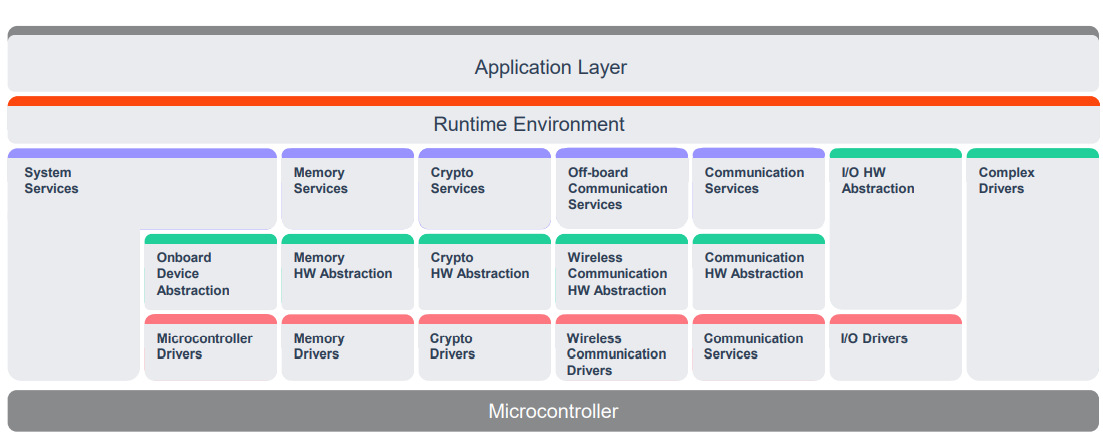
\includegraphics[width=1\textwidth]{imagens/classic platform.png}
  \captionsetup{justification=centering}
  \captionfont{\small{\textbf{\\Fonte: \cite{AUTOSAR}}}}  
  \label{fig:autoclassic}
\end{figure}


\begin{figure}[H]
  \setlength{\abovecaptionskip}{0pt} \setlength{\belowcaptionskip}{0pt}
  \caption{AUTOSAR Adaptive Platform}
  \centering
  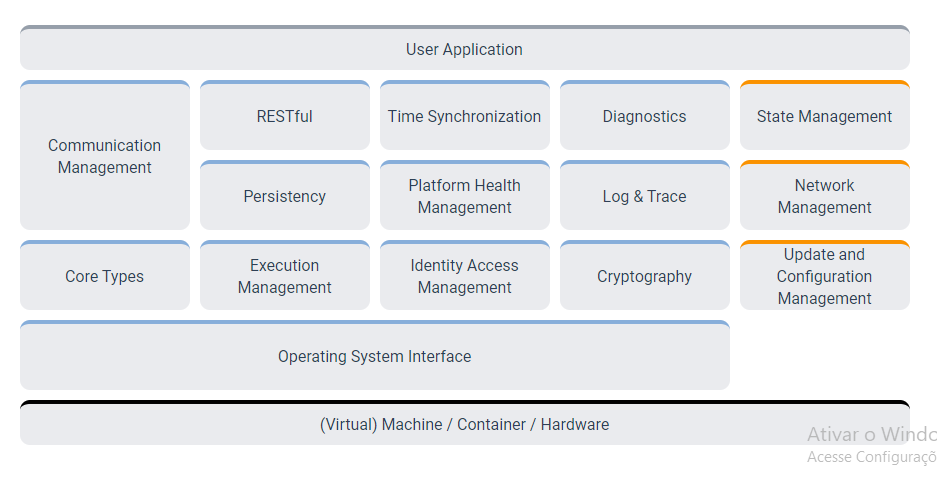
\includegraphics[width=1\textwidth]{imagens/adaptive platform.png}
  \captionsetup{justification=centering}
  \captionfont{\small{\textbf{\\Fonte: \cite{AUTOSAR}}}}  
  \label{fig:autoadaptive}
\end{figure}


\subsection{Robot Operating System}


The Robot Operating System (ROS), despite the name, it was not a operating system in the sense of scheduling and process management but actually a framework to facilitate the development of robotic applications. It needed to run on the top of an operating system providing interface for the users and the machine resources. Developing code for robots was hard due to its size and complexity. The code stack could reach the driver level going up to perception, mapping and reaching the user interface . Also the difference of hardware in each robot could make software reuse impossible without a common developing software \cite{quigley2009}. It was clear that robot development was not a single man task needed a cooperative effort to be developed. These were the main motivations to ROS framework development.

The base of the ROS schema was the Nodes, that were independent software structured in a graph way, remembering the object oriented programming, having some of its advantages. It promoted decoupling and reuse of ROS packages developed by the research community. ROS uses the publish and subscribe fashion for multiple nodes communication and request and response for peer to peer data request. It was able to record and play messages exchanged between nodes using the rosbag feature. It uses the Transmission Control Protocol (TCP) or the User Datagram Protocol (UDP) as a communication tool what enabled the work with distributed system meaning that several computers were seen as one big ROS system independently where the communication nodes are located \cite{ROS}. Furthermore, it was programmed using mostly C++ and Python programming languages.

\begin{figure}[H]
  \setlength{\abovecaptionskip}{0pt} \setlength{\belowcaptionskip}{0pt}
  \caption{Publish Subscriber Schema in ROS Nodes}
  \centering
  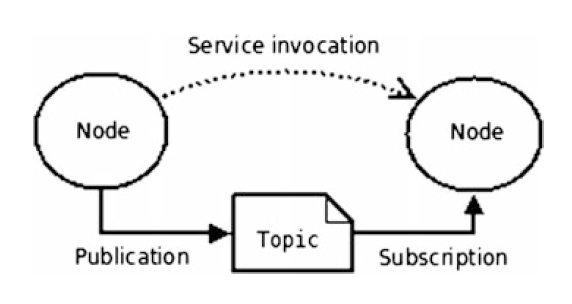
\includegraphics[width=1\textwidth]{imagens/ROSNodes.png}
  \captionsetup{justification=centering}
  \captionfont{\small{\textbf{\\Fonte: \cite{guettier2016}}}}  
  \label{fig:autonodes}
\end{figure}


Looking into the literature, ROS was the most used framework to develop robotic applications being the others frameworks such as AUTOSAR or Apollo based on that. However, when ROS was applied to the ADV, what could be called a special type of ROBOT, it was found some drawbacks. The ADV software system needed to have correct real time responses within a strict time window. Usually the overall system response could no be over 200 milliseconds. Using the TCP or UDP protocol could not guarantee real time response or correctness of the data transmitted through the communication channel what could be catastrophic. 

Furthermore, Valigi, N. \cite{valigi2018} cited some other challenges in developing autonomous vehicle software in ROS. The publish/subscribe pattern is the main issue bringing challenges even in a small scale projects. Inter process communication overhead without a shared memory, performance and reliability through multiple nodes communication over several machines, unnecessary coupling between framework and OS due to many OS-level processes created and the distributed programming mindset necessary even when its not the case were the main drawbacks pointed by the author. Liu et al \cite{Liu2019} also state that reliability as ROS did not monitore its nodes health and the unnecessary duplication of sended messages were issues that degraded the performance  The ROS community organized and developed the ROS 2 to face some of theses challenges. 

The main change in the ROS 2 was the implementation of the Data Distribution Protocol (DDS) substituting the TCP/UDP protocols. The DDS offers the advantage of a real-time data transmission support. Users could prioritize their threads and nodes without the need of a ROS Master thus reducing communication overhead \cite{stavrinos2021}. Another important improvement was the determinism of the execution order of the nodes that was not possible in ROS. ROS 2 was in development \cite{ROS} and even though it brought great improvements in the communication stack with DDS it still hold limitations. Specially the necessity to have a OS like Linux on top of it makes impossible to the whole system to have hard real time behaviour what was necessary for an ADV software system \cite{gutierrez2018} \cite{Reke2020}.

\subsection{Appolo Auto}
Apollo was an open source project from the chinese giant technology company Baidu that atracted several companies as partners. They aimed to provide an ADV software platform, sugested ADV hardware and simulation software with real data to test. Beginning the research in 2013, it was first tested in 2015 and became open for the community in 2017. \cite{Zhang2018} It started in the early versions as an extension of ROS. From the version 3.5 it was replaced by the Cyber RT framework that claimed to be more efficient than ROS itself using a lighter communication structure. Apollo provided many ADV necessary resources such as obstacle perception, route planning, cloud communication and HD maps \cite{Kessler2019} \cite{Liu2017}. 

\begin{figure}[H]
  \setlength{\abovecaptionskip}{0pt} \setlength{\belowcaptionskip}{0pt}
  \caption{Apollo System}
  \centering
  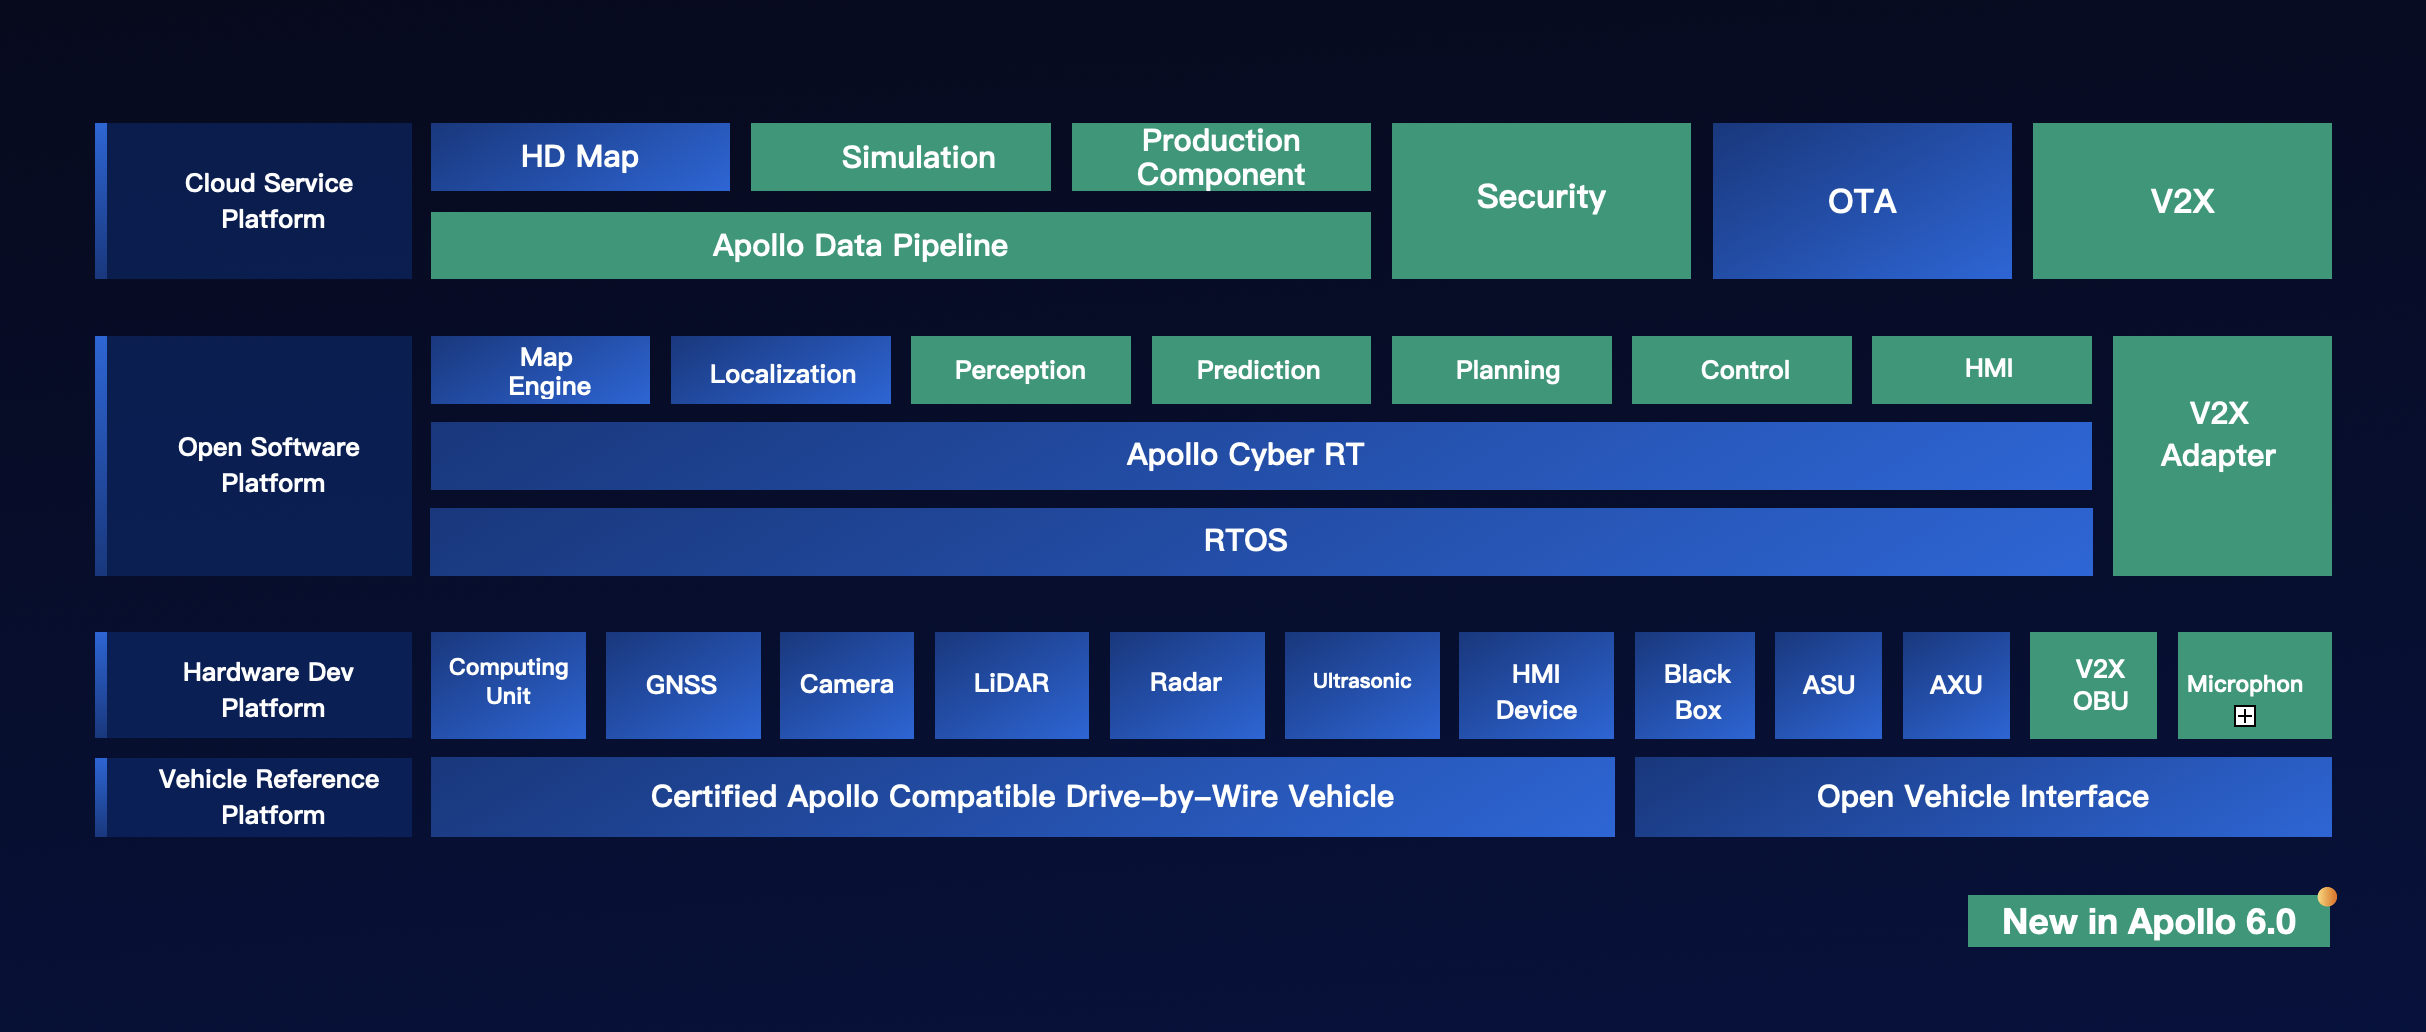
\includegraphics[width=1\textwidth]{imagens/Apollo_6_0.png}
  \captionsetup{justification=centering}
  \captionfont{\small{\textbf{\\Fonte: \cite{ApolloAuto}}}}  
  \label{fig:Apollo}
\end{figure}

The Apollo Kernel was a Linux modified kernel to run the Apollo software stack. It had real time capabilities and latest communication driver. At that time Apollo had already moved from development do productization wit many real applications in the world. Cyber RT was the Apollo framework designed specifically for ADV hardware and logic control. It was developed for a centralized computing architecture and built upon the concept of components\cite{Apollo}. It aimed to improve latency, concurrency and throughput in addition to accelerated development and accelerated deployment. The main innovation comparing to ROS was the possibility to use the RAM memory to transfer messages between modules. It was crucial for transferring messages with a lot of data without delays \cite{Buyval2019}.

Buyval et al. \cite{Buyval2019} found difficulties to use Apollo software, especially the path planning system. It used a multilevel approach with the data fed straight to the controller module. Between the disadvantages presented, the most relevant is that it took too long to process the trajectory. This made it impossible to be applied in a dynamic road scenario. Kessler at al. \cite{Kessler2019} needed to change drivers, include adapters and modify modules to apply the Apollo system in its ADV prototype. The author concludes that many barriers were encountered to use the Apollo System. 

\subsection{NVIDIA DRIVE}\label{ref:ml}

NVIDIA DRIVE was the proprietary solution designed by NVIDIA to control its ADV specific hardware. It was a software stack composed by a RTOS, middleware and software components directed to provide the ADV its necessary resources. It was part of the NVIDIA DRIVE System composed by simulators, software, training platform and was compatible with NVIDIA in-vehicle computers DRIVE AGX and DRIVE PX2. It aimed to deliver a safe and secure execution environment for hard real time applications with secure boot and services, firewall and over-the-air updates.


\begin{figure}[H]
  \setlength{\abovecaptionskip}{0pt} \setlength{\belowcaptionskip}{0pt}
  \caption{NVIDIA DRIVE system}
  \centering
  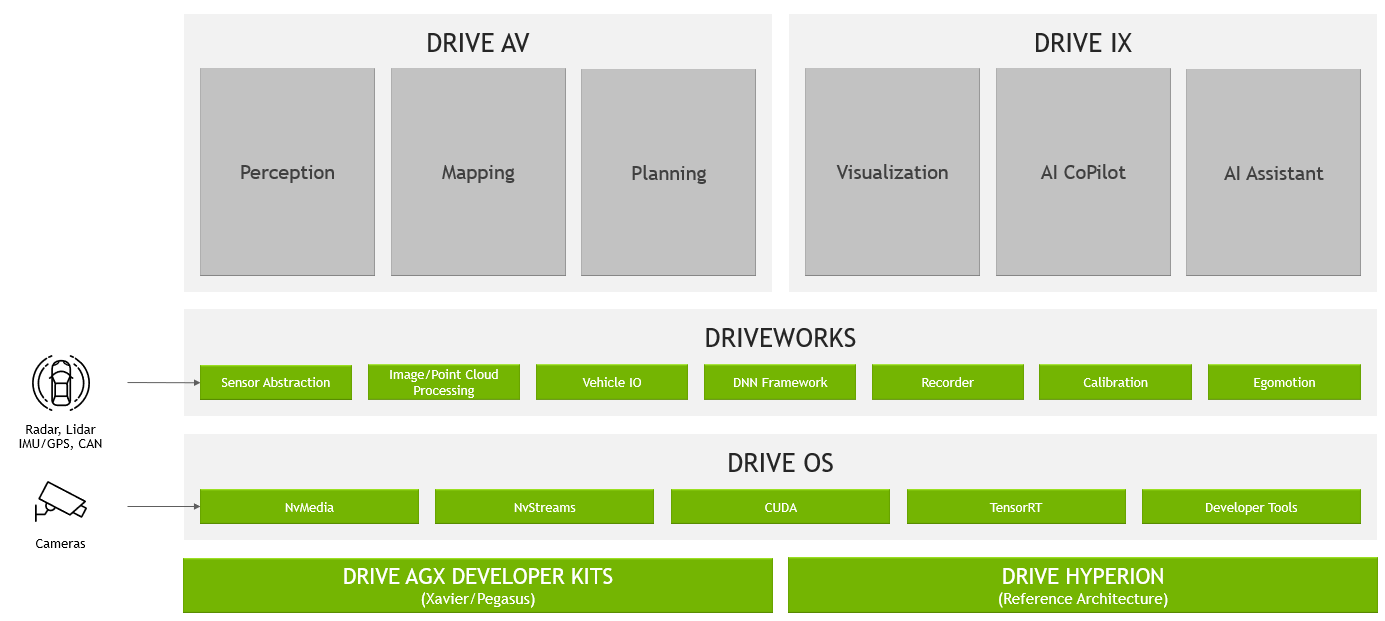
\includegraphics[width=1\textwidth]{imagens/driveworks.png}
  \captionsetup{justification=centering}
  \captionfont{\small{\textbf{\\Fonte: \cite{NvidiaDrive}}}}  
  \label{fig:NvidiaDRive}
\end{figure}

The NVIDIA DRIVE was divided in four parts. The DRIVE OS was the operating system of the stack that provided direct access to the hardware resources. It had a hard real time operating system embedded with the NVIDIA CUDA and TensorRT libraries. It also had a NVIDIA developed Hypervisor for guesting operating systems like Linux versions that provided access to the DRIVE OS itself. The NVIDIA DriveWorks was the midlleware that provided all the necessary libraries modules for ADV specific applications. It dealt with tasks such as sensor signals collection, image and point cloud processing, deep neural networks models and Vehicle IO collection. This middleware ready made components had the objective to use the maximum throughput available on the NVIDIA hardware in use.

On the top of the stack, the DRIVE AV provided the algorithms and strategies for perception, mapping and planning in separated modules. It was accessed using the DRIVE WORKS development interface. It module had an extensive list of resources treated as a separated software component. The last part of the system was the DRIVE IX. It supplied human machine interface and specific features aimed to the interaction with the driver on the vehicle cabinet. It enabled the development of applications such as driver conditions aid, system visualization, voice and face recognition

Researchers have proposed various approaches to optimize task scheduling, including middleware solutions that facilitate data transmission and process management, intelligent scheduling algorithms that dynamically allocate resources, and AI-based strategies that use machine learning for enhanced adaptability and efficiency. This section provides an overview of the existing literature on task scheduling for autonomous vehicles, focusing on both traditional scheduling frameworks and AI-driven techniques.
\subsection{Task Scheduling for Autonomous Vehicles}

The Cocktail Project \cite{Zong2018} was designed to overcome the drawbacks of ROS when dealing with real-time systems. It is a general purpose middleware focused on data transmission. It is used to control communications between the many processes running in an ADV system. It deals with the data as binary streams that are free from any data format of the processes peers. In this project, an intelligent task scheduler called IoThreadPool was introduced. When the IO data from the ADV sensors are collected, this scheduler decides on the best strategy. It could be creating new threads or using threads already available. It also assigns the best available processor to the thread to maximize throughput.

PI-Edge \cite{tang2018} is a computing framework designed to efficiently handle multiple tasks in autonomous heterogeneous computing systems. It was composed of a runtime layer with a scheduler developed in OpenCL. Dynamically dispatches incoming tasks to the best suitable processing unit available. It consists of two layers. The intercore scheduler is the first barrier that receives incoming tasks and assigns them to the computing units based on availability and task affinity. It uses a variation of the Min-Min algorithm developed by the author called Dif-Min. It could obtain an average 10\% reduction in makespan compared to the Min-Min algorithm. The inner-core scheduler organizes the tasks queue inside the same processor based on task priority and dependency between them. It uses the table-based heterogeneous earliest finish time as a scheduling algorithm.

\cite{amarnath2021}  proposed a two level scheduler called HetSched. One level named Meta-Sched processes the DAG dependencies. Verifies if a task is ready to be executed if there is no parent task to be executed on the graph. It also elects DAGs to not be executed due to the unfeasible deadlines of its tasks.  The ready tasks are handled by the Task-Sched that actually delivers tasks to the processing units that can process it. The scheduler ranked the tasks to be executed using its earliest finish time. It was calculated using its execution time, processing unit status, and the task queue scheduled to the same processing unit. The scheduler was tested on a Jetson TX1 board composed of GPU accelerators and CPU processors. The tasks used to test were from two benchmark suites that simulate a simplified autonomous vehicle. Based on the experimental results, it was possible to determine the best configuration of computing units for urban scenarios based on the experimentation.

\subsection{AI-Based Task Scheduling for ADVs}

\cite{Balasekaran2021}  proposed an intelligent task management system for autonomous driving. It was composed of a resource predictor using a single-layer feedforward neural network and a scheduler using the hyper period first algorithm. It was developed in Python and tested on a multicore system consisting of an Odroid XU4 and NVIDIA Jetson embedded platforms. When put against the Connected Autonomous Vehicles and Internet of Medical Things benchmarks it achieved 98\% better accuracy, reduction between 20\% to 27\% of execution time and 32\% to 45\% reduction in task miss rate compared with conventional task scheduling methods.

Furthermore, Xu et al. \cite{Xu2022} propose the Age of Information (AoI)-centric task scheduling approach that aims to ensure that tasks use the most recent sensor data, which is critical for correct detection, planning, and action taking by ADV. The schedule uses a reinforcement learning solution by integrating its scheduler with a DDQN to solve hard combinatorial problems. 

Many recent researches believe that autonomous vehicles would not be able to handle all the computational load required to drive autonomously due to their limited computational resources \cite{qi2020, dai2019, lin2019, liu2019task}. Hence, the use of mobile edge computing servers (MECS) would be necessary to unload autonomous driving tasks from the ADV to the servers. This assumption would become feasible with the 5G network deployment. Therefore, to take advantage of the available edge computing infrastructure, it is necessary to gracefully schedule ADV tasks based on its priorities and characteristics to the most suitable and available MECS. 

Inquiring that the full system, composed of ADV and MECS interconnected by a wireless network, could not be mathematically modeled accurately, \cite{qi2020,liu2019task} proposed the use of a DRL approach to distribute the incoming ADV tasks to the MECSs in a parallel fashion. A set of characteristics from the task are extracted and used as a input for the DRL algorithm that after some training epochs starts to deliver the optimal solution for scheduling the task to the available nodes. Both authors compared their results with well-known scheduling algorithms for heterogeneous computing systems that proved to bring some average processing time reduction to the ADV computing system.

Organizing and scheduling real time tasks responsible for the ADV action-taking process was the objective of \cite{lin2019}. Hence, a reinforcement learning algorithm based on simulated annealing (SA-RL) was proposed to improve system performance. The authors suppose that the tasks would be transferred to edge computing nodes instead of being processed inside the vehicle computing system. The scheduler was designed according to the difference in tasks and sub tasks and changes in the edge computing environment. The problem was described using a Markov decision process, and the completion time was calculated using an algorithm devised by the author. Afterward, a Q-learning algorithm based on simulated annealing was applied to improve the task completion rate. Finally, the proposed SA-RL algorithm was simulated on a computer with a Windows 10 operating system against the particle swarm optimization algorithm. Both algorithms performed well in feasibility and effectiveness; however, the authors' strategy converged faster and maintained a low level of fluctuation with respect to the average completion time.


\end{comment}
